\documentclass[10pt]{article}

\usepackage[margin=1in]{geometry}
\usepackage{amsmath,amssymb}
\usepackage{graphicx}
\usepackage{booktabs}
\usepackage{microtype}
\usepackage[numbers,sort&compress]{natbib}
\usepackage{xcolor}
\usepackage[colorlinks=true,linkcolor=blue!60!black,citecolor=blue!60!black,urlcolor=blue!60!black]{hyperref}
\usepackage{caption}
\captionsetup{font=small,labelfont=bf}

\newcommand{\loss}{\mathcal{L}}
\newcommand{\R}{\mathbb{R}}

\title{Differentiable Minkowski Functionals for Neural Fields:\\
Validation, Design Rules, and an Adversarial Failure Mode}

\author{Gunner Levi Howe\\
Independent Researcher\\
\texttt{gunnerlevihowe@gmail.com}}

\date{July 2026}

\begin{document}
\maketitle

\begin{abstract}
The Minkowski functionals of a field's excursion sets---area, boundary measure, and
Euler characteristic---are the complete integral-geometric description of its
level-set morphology, and the Euler characteristic is the cheapest handle on its
\emph{topology}. We derive smooth Monte-Carlo estimators for all three functionals of
a continuous neural field, evaluated at scattered sample points via the co-area
formula and the Gauss--Bonnet theorem, using only automatic differentiation: no grid,
no simplicial or cubical complex, no persistence computation. The Euler-characteristic
estimator is accurate to $1$--$3\%$ against exact topology in 2D and 3D (bumps,
merges, holes, handles) at $2\times10^5$ samples, and costs $\sim$3\,ms per training
iteration where a persistent-homology (PH) loss on a cubical grid costs
$\sim$650--1000\,ms---a $250\times$ gap. We establish four design rules without which
these losses silently fail: a dense \emph{level ladder} (topological invariants are
almost-everywhere flat in the parameters; gradients exist only near transitions), a
$C^2$ \emph{backbone} (ReLU networks hide curvature in kinks invisible to sampling),
the full \emph{Minkowski vector} (the Euler characteristic alone is an alternating sum
and is gamed by debris--hole cancellation; pricing perimeter closes the channel), and
\emph{sampling-scale coverage}. In 2D, the resulting vector-valued cap is the only
method in a controlled comparison that both repairs topology (3/3 seeds) and preserves
signal fidelity---uniform smoothing repairs at $11$--$17\times$ the fidelity cost, and
the Euler term alone repairs nothing. In 3D neural-SDF fitting, however, we measure a
failure mode we believe generalizes to any sampled soft topology objective: gradient
descent adversarially concentrates topological noise \emph{below the sampling
density}, where the estimator and its guards are provably blind---spurious-feature
counts are invariant to a $4\times$ increase in samples, and closing the blind window
requires cubically many points, erasing the cost advantage. A grid-based PH baseline,
whose complex \emph{is} the evaluation resolution, solves the same benchmark
(4/9 exact topology; median $b_1$ error 1 vs.\ ours $>10^4$). We conclude that the
$250\times$ cost of persistence is, at present, the price of having no null space, and
we release estimators, receipts, and benchmarks.
\end{abstract}

\section{Introduction}
\label{sec:intro}

Controlling the topology of a learned implicit shape---``one component, two handles,
no cavities''---is a recognized open problem: the persistent-homology (PH) literature
itself notes that classical invariants such as Betti numbers ``are not easily used''
as direct controls in implicit surface reconstruction \citep{dong2022topologycad}, and
the state of the art constrains topology through persistence diagrams computed on
cubical complexes at every training step \citep{stitch2024}. That machinery is
powerful but expensive and grid-bound.

Integral geometry offers a lighter-looking route. For a smooth field
$f:\Omega\subset\R^d\to\R$ and excursion sets $A_u=\{f\ge u\}$, the Minkowski
functionals---in 2D: area $M_0(u)$, boundary length $M_1(u)$, Euler characteristic
$M_2(u)=\chi(A_u)$---admit \emph{integral representations} that require neither a grid
nor a complex. This paper asks, and answers with pre-registered gates and kill
conditions, the natural question: can those representations be turned into
differentiable training objectives for neural fields, and do they displace
persistence?

This is the third study in a program that turned the Kac--Rice level-crossing density
(exactly $M_1$) into a spectral-bias loss for implicit neural representations
\citep{howe2026levelcrossing} and a one-sided stabilizer budget for physics-informed
networks \citep{howe2026budget}. The answer here has the same honest shape as those
papers: the machinery is real, validated, and fast; its working domain is real but
bounded; and the boundary itself is the most instructive result.

\paragraph{Contributions.}
(1)~\emph{Estimators}: smooth Monte-Carlo Minkowski profiles of continuous neural
fields at scattered points (Section~\ref{sec:method}), with the Euler characteristic
via a Gauss--Bonnet/co-area integrand in 2D and 3D, validated to $1$--$3\%$ against
exact topology (Table~\ref{tab:gatev}) at $\sim$3\,ms per training iteration.
(2)~\emph{Design rules}, each discovered through a documented failure: the level
ladder, the $C^2$ backbone, the Minkowski-vector defense, and sampling-scale coverage
(Section~\ref{sec:rules}).
(3)~\emph{A controlled 2D success}: the vector-valued cap is the only method in a
four-way comparison that repairs topology on every seed while preserving fidelity
(Table~\ref{tab:exp9}).
(4)~\emph{A measured 3D failure mode}: sampled topology losses are adversarially
exploitable in their sub-sampling null space; the debris is invariant to affordable
increases in sampling, while a faithful PH baseline solves the benchmark at
$250\times$ the per-iteration cost (Table~\ref{tab:exp10},
Figure~\ref{fig:scaling}).

\paragraph{What we do not claim.} Differentiable Euler-characteristic machinery
exists for discrete complexes \citep{roell2024dect}, statistical shape transforms
\citep{marsh2022sect}, and pixel grids \citep{minkloss2026}; PH losses for implicit
surfaces exist \citep{stitch2024,dong2022topologycad}; curvature energies for neural
SDFs exist \citep{neurcadrecon2024,gropp2020igr}. Our claim is confined to the
continuous-field, complex-free, scattered-point instantiation---and we show its
current 3D limit as prominently as its 2D success.

\section{Method}
\label{sec:method}

\paragraph{Estimators.} With a Gaussian bump
$\delta_\varepsilon(z)=(2\pi\varepsilon^2)^{-1/2}e^{-z^2/2\varepsilon^2}$ and samples
$x_1,\dots,x_N$ covering $\Omega$ (volume $V$), the co-area formula gives
\begin{align}
\hat M_0(u) &= \tfrac{V}{N}\textstyle\sum_i \sigma\!\big((f(x_i)-u)/\varepsilon\big),
\qquad
\hat M_1(u) = \tfrac{V}{N}\textstyle\sum_i
\delta_\varepsilon(f(x_i)-u)\,\lVert\nabla f(x_i)\rVert,
\label{eq:m01}
\end{align}
and, for the Euler characteristic, Gauss--Bonnet on the level set: in 2D,
$\chi(A_u)=\frac{1}{2\pi}\oint_{\partial A_u}\kappa_g\,ds$ with
$\kappa_g=-\mathrm{div}(\nabla f/\lVert\nabla f\rVert)$, hence
\begin{equation}
\hat\chi(u) \;=\; -\frac{V}{2\pi N}\sum_i
\delta_\varepsilon(f(x_i)-u)\,
\frac{f_{xx}f_y^2 - 2f_{xy}f_xf_y + f_{yy}f_x^2}{\lVert\nabla f(x_i)\rVert^{2}},
\label{eq:chi2d}
\end{equation}
and in 3D, via $\int_S K\,dA = 2\pi\chi(S)$ and $\chi(\text{solid})=\chi(S)/2$ with
Goldman's implicit-surface Gaussian curvature \citep{goldman2005curvature},
$\hat\chi(u) = \frac{V}{4\pi N}\sum_i \delta_\varepsilon(f_i-u)\,
\nabla f_i^{\!\top}\mathrm{adj}(H_i)\nabla f_i / \lVert\nabla f_i\rVert^{3}$.
All derivatives come from automatic differentiation; the sign conventions are fixed
by the unit-disc case and verified in released unit tests. Losses match or one-sidedly
cap the profile vector at $L$ fixed levels with the relative normalization of the
companion papers.

\paragraph{Validation.} Table~\ref{tab:gatev}: on analytic fields with
hand-verifiable excursion topology---including the sign-critical annulus ($\chi=0$)
and solid torus ($\chi=0$)---the estimator is exact to within $1$--$3\%$ with
seed-level standard deviations below $0.08$, in both dimensions, at
$N=2\times10^5$. As a \emph{measurement}, the tool is settled.

\begin{table}[t]
\centering
\caption{\textbf{Estimator validation} (3 seeds, $N=2\times10^5$,
$\varepsilon=0.02$). Fields decay below probed levels at the domain boundary, so no
Gauss--Bonnet boundary terms arise.}
\label{tab:gatev}
\begin{tabular}{lccc}
\toprule
Field & exact $\chi$ & $\hat\chi$ range (3 seeds) & s.d. \\
\midrule
2D one bump & 1 & 0.998--1.021 & $\le 0.012$ \\
2D two bumps (merge) & 2 / 1 & 2.005--2.017 / 1.006 & $\le 0.026$ \\
2D annulus (hole) & 0 & 0.011--0.019 & $\le 0.040$ \\
3D ball & 1 & 0.987--1.012 & $\le 0.019$ \\
3D solid torus & 0 & 0.016--0.026 & $\le 0.071$ \\
\bottomrule
\end{tabular}
\end{table}

\section{Four design rules, four documented failures}
\label{sec:rules}

Each rule below was forced by an experiment that failed without it; the receipts (run
logs and seeds) ship with the code.

\paragraph{Rule 1: the level ladder.} $\chi(A_u)$ is a topological invariant, hence
piecewise-constant in the network parameters; a smoothed estimator supplies gradients
only within $\sim\varepsilon$ of a topology-changing event. A cap probing levels
$[0.1,0.4]$ against a spurious feature peaking at $0.7$ received \emph{exactly zero
loss for 2{,}000 iterations}. Dense levels with spacing $\lesssim\varepsilon$ spanning
the value range form a ratchet: the topmost active level always sits near the
offending peak and supplies a live extinction gradient.

\paragraph{Rule 2: the $C^2$ backbone.} On a ReLU network (with smooth positional
encoding) the almost-everywhere Hessian omits the distributional curvature
concentrated at activation kinks; the sampled Gauss--Bonnet integral then
systematically under-counts and the loss never activates. On a SIREN backbone the
same estimator reads the same field's topology correctly. Smooth activations are a
requirement, not a preference---consistent with standard practice for curvature
losses \citep{gropp2020igr,neurcadrecon2024}.

\paragraph{Rule 3: the Minkowski vector.} $\chi$ is an alternating sum, so a
$\chi$-cap is satisfiable by \emph{cancellation}: in our runs the optimizer
manufactured four components and three holes ($\chi=1$, as demanded) rather than
deleting the one spurious component. Capping $M_1$ simultaneously prices the
cancellation channel---debris costs perimeter---after which honest deletion is the
cheapest descent path. The vector, not the invariant, is the loss.

\paragraph{Rule 4: sampling-scale coverage.} All three estimators are blind to
features smaller than the sample spacing. Rule~4 is the one that cannot be satisfied
affordably in 3D, and Section~\ref{sec:sdf} measures the consequence.

\section{Controlled 2D comparison: the vector cap works}
\label{sec:invitro}

A SIREN field is polluted with a spurious component, then repaired under an anchor on
clean-signal samples plus one of four regularizers; ground truth topology is read from
a $256^2$ grid, never from the estimator itself. Table~\ref{tab:exp9}: the anchor
alone never repairs; Hessian smoothing repairs 2/3 but pays $11$--$17\times$ in
fidelity when it does (same-seed MSE ratios $17.0$ and $11.5$; it smears the signal
along with the blob); the $\chi$-cap alone
repairs 0/3 (Rule~3's cancellation, observed on every seed); the vector cap repairs
\textbf{3/3} with the best or near-best fidelity throughout, and drives the spurious
region below the lowest probed level. In 2D---where $12$k samples resolve everything a
$256^2$ evaluation can see---the method does exactly what it promises.

\begin{table}[t]
\centering
\caption{\textbf{2D topology repair} (3 seeds; grid-verified). ``Repaired'' means
(1~component, 0~holes) at every probed level.}
\label{tab:exp9}
\begin{tabular}{lccc}
\toprule
Config & repaired & spurious max & clean MSE \\
\midrule
anchor only & 0/3 & 0.698 $\pm$ 0.092 & 0.0284 $\pm$ 0.0196 \\
+ smoothness (null) & 2/3 & 0.129 $\pm$ 0.010 & 0.0392 $\pm$ 0.0262 \\
+ $\chi$-cap alone & 0/3 & 0.355 $\pm$ 0.219 & 0.0057 $\pm$ 0.0037 \\
+ Minkowski-vector cap (ours) & 3/3 & 0.109 $\pm$ 0.001 & 0.0041 $\pm$ 0.0010 \\
\bottomrule
\end{tabular}
\end{table}

\section{3D neural SDFs: an adversarial failure mode}
\label{sec:sdf}

\paragraph{Benchmark.} SIREN SDFs fitted to $2{,}000$ noisy surface samples with
$5\%$ uniform outliers, for a sphere, torus, and genus-2 solid; Eikonal and anchor
losses throughout; topology read as voxel Betti numbers at $96^3$ (verified exact on
the analytic shapes); Chamfer distance to the clean surface; 3 seeds. Baselines:
Eikonal only, Hessian smoothing, our vector match, and a faithful cubical-complex PH
loss in the STITCH spirit \citep{stitch2024} via GUDHI \citep{gudhi}, differentiable
through its critical-cell values. Two regimes: a hard one
($\omega_0{=}15$, 8k collocation points) and a bandwidth-matched one
($\omega_0{=}8$, Eikonal weight $1.0$, 16k points). The PH configuration runs at half
the iterations---its per-iteration cost is $\sim$250$\times$ ours---and both
matched-iteration and matched-wall-clock readings favor the conclusions below.

\begin{table}[t]
\centering
\caption{\textbf{3D SDF benchmark} (3 shapes $\times$ 3 seeds per regime; ``topo
correct'' = exact Betti numbers $(b_0,b_1,b_2)$ at $96^3$). PH runs at half
iterations; its topo cost is per-iteration.}
\label{tab:exp10}
\begin{tabular}{lcccc}
\toprule
Config & topo correct & median $b_1$ err & Chamfer & topo ms/iter \\
\midrule
\multicolumn{5}{l}{\emph{hard ($\omega{=}15$, 8k) regime}} \\
Eikonal only & 0/12 & 390 & 0.239 & 0.0 \\
+ smoothness & 0/12 & 276 & 0.221 & 0.2 \\
+ Minkowski vector (ours) & 0/12 & 5734 & 0.275 & 3.1 \\
+ persistent homology & 1/12 & 4 & 0.188 & 828.3 \\
\midrule
\multicolumn{5}{l}{\emph{matched ($\omega{=}8$, 16k) regime}} \\
Eikonal only & 0/9 & 161 & 0.204 & 0.0 \\
+ smoothness & 0/9 & 81 & 0.210 & 0.1 \\
+ Minkowski vector (ours) & 0/9 & 91390 & 0.256 & 2.7 \\
+ persistent homology & 4/9 & 1 & 0.260 & 654.3 \\
\bottomrule
\end{tabular}
\end{table}

\paragraph{Result.} In the hard regime every method fails topologically---including
PH (1/12)---establishing that the benchmark is genuinely difficult. In the matched
regime PH separates: 4/9 exact (3/3 on the sphere) with median $b_1$ error 1. Our
vector match does not merely fail there; it fails \emph{spectacularly}. Throughout,
``spurious features'' means the summed Betti excess $b_0{+}b_1{+}b_2$ over ground
truth at the $96^3$ evaluation: the vector match accumulates $\sim$$1.7\times10^5$ in
total, of which $\sim$$7\times10^4$ are components ($b_0$) and the table's median
$b_1$ error alone exceeds $9\times10^4$---one field, three views of the same debris.

\paragraph{Diagnosis: the null space is found, not stumbled into.} Three facts
localize the mechanism. First, the debris is loss-induced: Eikonal-only runs show
2--3 orders of magnitude fewer features. Second, the debris lives at the voxel scale
($\sim$0.02), strictly below the collocation spacing ($0.05$--$0.08$): precisely
where $\hat\chi$, and the $M_1$ guard of Rule~3, receive no samples and hence no
gradient. Gradient descent, asked to satisfy a topology target it cannot honestly
reach quickly, discovers the estimator's blind window and hides topological noise
inside it---an adversarial attack by the optimizer on its own objective. Third, and
decisive: the debris count is \emph{invariant} to a $4\times$ increase in samples
(Figure~\ref{fig:scaling}); spacing falls from $0.08$ to $0.05$ while the window to
$0.02$ remains open. Closing it requires $N\sim(2/0.02)^3\approx10^6$ points, whose
Hessian evaluations would consume the entire $250\times$ cost advantage. The
grid-based PH loss has no such window---its complex \emph{is} the evaluation
resolution---and that, we conclude, is what its cost currently buys.

\begin{figure}[t]
\centering
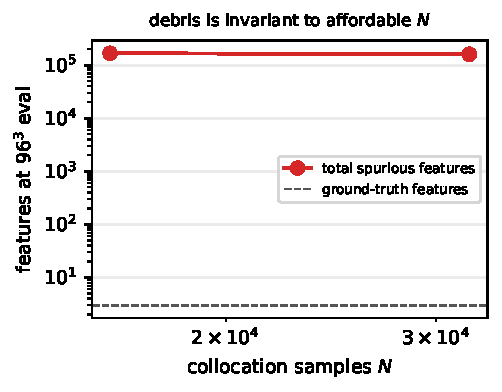
\includegraphics[width=.5\linewidth]{figs/p3_scaling.pdf}
\caption{\textbf{The blind window does not close affordably.} Total spurious
features of the vector-match SDF (median over shapes, seed 0, matched regime) versus
collocation samples $N$: flat where a sampling-resolution mechanism would require
decay, because the debris relocates below whatever spacing is affordable.}
\label{fig:scaling}
\end{figure}

\section{Related work}
\label{sec:related}

Differentiable Euler-characteristic transforms operate on simplicial/cubical data
\citep{roell2024dect}; smooth Euler characteristic transforms serve statistical shape
inference \citep{marsh2022sect}; differentiable Minkowski surrogates exist for pixel
grids via relaxed morphology \citep{minkloss2026}. Topology control for implicit
surfaces is dominated by persistence \citep{stitch2024,dong2022topologycad}.
Curvature-based (non-topological) energies for neural SDFs include the Eikonal term
\citep{gropp2020igr}, its divergence-stabilized refinement \citep{yang2023steik}, and
zero-Gaussian-curvature CAD priors \citep{neurcadrecon2024}. On the theory side, the
\emph{expected} Minkowski functionals of Gaussian-related fields are the subject of
the Gaussian kinematic formula \citep{adler2007random,azais2009level}---the same
random-field-theory lineage as the Rice formula that seeded this program; our
estimators are its deterministic, per-field, trainable counterpart. The
co-area/Gauss--Bonnet Monte-Carlo route for \emph{continuous neural fields at
scattered points}, and its use as a training loss, is to our knowledge new here---as
is the negative half of its characterization. The estimators extend the Kac--Rice
program of \citep{howe2026levelcrossing,howe2026budget}, whose $M_1$ machinery this
paper reuses verbatim as the Rule-3 guard.

\section{Discussion and limitations}
\label{sec:discussion}

\paragraph{When to use which tool.} As a \emph{measurement} on smooth fields, the
Minkowski profiles are accurate, differentiable, dimension-agnostic, and essentially
free; we expect them to be useful as diagnostics and evaluation statistics well beyond
losses (the companion papers' crossing-profile diagnostic is the $M_1$ special case).
As a \emph{training loss}, the validated domain is: smooth backbone, dense level
ladder, full vector, and sampling that covers the evaluation scale---conditions met in
our 2D setting and unmet, affordably, in 3D. Where they cannot be met, persistence on
a complex at evaluation resolution remains the tool of record.

\paragraph{Open routes for 3D.} The failure is a sampling-allocation problem, not an
estimator error: uniform collocation wastes almost all samples away from level sets.
Importance sampling concentrated near $\{f\approx u\}$, multi-resolution ladders,
debris-seeking adversarial samplers, or hybrid schemes (cheap Minkowski steps
punctuated by sparse PH corrections) are all plausible; none are tested here, and we
make no claims about them.

\paragraph{Limitations.} Boundary terms are dodged by construction (fields decay at
the domain edge); levels are fixed rather than adaptive; the PH baseline is our
faithful-in-spirit reimplementation rather than released STITCH code; shapes are
analytic solids rather than scanned geometry; and all wall-clock figures come from one
workstation.

\section{Conclusion}

We set out to displace persistent homology with integral geometry and did not.
What stands instead: a validated, $250\times$-cheaper family of differentiable
topological observables for neural fields; four transferable design rules, each
carrying the failure that forced it; a controlled setting where the approach is the
only one that works on both axes; and a precisely measured adversarial mechanism---
optimizers hunt the null space of sampled objectives---that we believe any future
sampled topology loss must answer. The boundary between the geometry that sampling
can police and the topology that requires a complex is now measured, not conjectured.

\paragraph{Reproducibility.} Code, unit tests (sign conventions, exact-topology
validation, gradient flow), all raw run JSONs, and the failure-receipt logs:
\url{https://github.com/gunnerhowe/Research} (directory \texttt{kac-rice};
estimators in \texttt{src/kacrice/minkowski.py}, SDF harness in
\texttt{src/kacrice/sdf.py}, suites in \texttt{experiments/run\_phase3.py}, figures
via \texttt{experiments/make\_figures\_phase3.py}). Environment: Python 3.13.6,
PyTorch 2.7.1, NumPy 2.4.4, SciPy 1.17.0, GUDHI 3.13.0, scikit-image 0.26.0; one
consumer workstation (16-core CPU / RTX~3080). Seeds $0$--$2$ throughout (seed $0$
for the sampling sweep); every table regenerates from
\texttt{results/phase3/*.json}.

\bibliographystyle{plainnat}
\bibliography{references}

\end{document}
